% \usepackage[table]{xcolor}
% \usepackage{graphicx}
% \usepackage{hyperref}
% \usepackage{listings}
% \usepackage{pifont}
% \usepackage{balance}
% \usepackage{booktabs}
% \usepackage{arydshln}
% \usepackage{wrapfig}
% \usepackage[firstpage]{draftwatermark}
\graphicspath{{chap3/images/}}

%% artifact evaluation badge
%% adjust the two parameters to change the location
% \SetWatermarkText{\raisebox{11.5cm}{%
% 		\hfill \hspace{8.4375cm} \includegraphics{2-functional}%
% }}
% \SetWatermarkAngle{0}

\newcommand{\ra}[1]{\renewcommand{\arraystretch}{#1}}

\newcommand{\cmark}{\ding{51}\xspace}
\newcommand{\xmark}{\ding{55}\xspace}
\newcommand{\notapplic}{N/A\xspace}

% \newcommand{\shaobo}[1]{\textcolor{green}{Shaobo sayz: #1}}
% \newcommand{\zvon}[1]{\textcolor{red}{Zvon sayz: #1}}
% \newcommand{\marek}[1]{\textcolor{green}{Mark sayz: #1}}
% \newcommand{\jj}[1]{\textcolor{green}{JJ sayz: #1}}

\renewcommand{\ttdefault}{pxtt}

\lstdefinelanguage{boogie}{%
  keywords={%
    procedure,var,int,call,return,assert,
  },
  morecomment=[l]{//},
}

\lstdefinelanguage{llvm}{%
  keywords={%
    define,void,alloca,call,bitcast,store,align,to,load,ret,void,getelementptr,icmp,
    inbounds,eq,
  },
  morecomment=[l]{//},
}

\lstdefinelanguage{swift}
{
  morekeywords={
    func,if,then,else,for,in,while,do,switch,case,default,where,break,continue,fallthrough,return,
    typealias,struct,class,enum,protocol,var,func,let,get,set,willSet,didSet,inout,init,deinit,extension,
    subscript,prefix,operator,infix,postfix,precedence,associativity,left,right,none,convenience,dynamic,
    final,lazy,mutating,nonmutating,optional,override,required,static,unowned,safe,weak,internal,
    private,public,is,as,self,unsafe,dynamicType,true,false,nil,Type,Protocol,Int
  },
  morecomment=[l]{//}, % l is for line comment
  morecomment=[s]{/*}{*/}, % s is for start and end delimiter
  morestring=[b]" % defines that strings are enclosed in double quotes
}

\lstdefinelanguage{rust}{%
  keywords={%
    fn,i1,i8,u8,i16,u16,i32,u32,i64,u64,mut,for,in,as,match,struct,let,mod,use,
    pub,extern,unsafe,bool,if,return,usize
  },
  morecomment=[l]{//},
}

\lstset{
  breaklines=true,
  postbreak=\mbox{\textcolor{red}{$\hookrightarrow$}\space},
}

% \newcommand{\lstc}[1]{\lstset{language=C,basicstyle=\ttfamily\footnotesize}\lstinline´#1´}
% \newcommand{\lstrust}[1]{\lstset{language=rust,basicstyle=\ttfamily\footnotesize}\lstinline´#1´}
\newcommand{\lstswift}[1]
{\lstset{language=swift}\lstinline?#1?}
% The above used to have a `´' instead of `?', but none of the examples in this text use the `?', so we'll use that instead to avoid unicode errors.
%\newcommand{\lstswift}[1]{\lstset{language=swift,basicstyle=\ttfamily\footnotesize}\lstinline´#1´}
% \newcommand{\lstllvm}[1]{\lstset{language=llvm}\lstinline´#1´}
% \newcommand{\lstboogie}[1]{\lstset{language=boogie}\lstinline´#1´}
% \newcommand{\rustc}{{rustc}}


% \begin{document}
\chapter[Leveraging Compiler Intermediate Representation for\\Multi- and
Cross-Language Verification]{Leveraging Compiler Intermediate Representation for Multi- and
Cross-Language Verification\protect\footnotemark} \footnotetext{Adapted from \textit{Leveraging Compiler Intermediate Representation for Multi- and Cross-Language Verification}, VMCAI 2020~\cite{2020_vmcai_gbhr}. Reproduced with permission from Springer Nature.}
\label{cha3}
\setupuuchapterbib
% \thanks{This work was supported by funding from the
% Undergraduate Research Opportunities Program at the University of Utah awarded
% to Jack J.~Garzella, the National Science Foundation awards CNS 1527526 and CCF
% 1837051, and a gift from the VMware's University Research Fund.}}

% \titlerunning{Leveraging Compiler IR for Multi- and
% Cross-Language Verification}

% \author{Jack J.~Garzella \and Marek Baranowski \and Shaobo He \and Zvonimir Rakamari\'c}
% \institute{
%   School of Computing, University of Utah \\
%   Salt Lake City, UT, USA \\
%   \email{jjgarzella@gmail.com,\\
%   \{baranows,shaobo,zvonimir\}@cs.utah.edu}
% }

% \authorrunning{J.~J.~Garzella \and M.~Baranowski \and S.~He \and Z.~Rakamari\'c}

% \maketitle
%\marek{Is the lncs abstract necessary in this? It seems redundant with the introduction. The thesis template says implies it's rude to not have text here though.}
% \begin{abstract}
% %
% Developers nowadays regularly use numerous programming languages with different
% characteristics and trade-offs.
% %
% Unfortunately, implementing a software verifier for a new language from scratch
% is a large and tedious undertaking, requiring expert knowledge in multiple
% domains, such as compilers, verification, and constraint solving.
% %
% Hence, only a tiny fraction of the used languages has readily available
% software verifiers to aid in the development of correct programs.
% %
% In the past decade, there has been a trend of leveraging popular compiler
% intermediate representations (IRs), such as LLVM IR, when implementing software
% verifiers.
% %
% Processing IR promises out-of-the-box multi- and cross-language
% verification since, at least in theory, a verifier ought to be able to handle a
% program in any programming language (and their combination) that can be
% compiled into the IR.
% %
% In practice though, to the best of our knowledge, nobody has explored the
% feasibility and ease of such integration of new languages.
% %
% In this paper, we provide a procedure for adding support for a new
% language into an IR-based verification toolflow.
% %
% Using our procedure, we extend the SMACK verifier with prototypical support for
% 6 additional languages.
% %
% We assess the quality of our extensions through several case studies, and we
% describe our experience in detail to guide future efforts in this area.
% %
%\keywords{Verification \and Multi-Language \and Cross-Language \and Compiler
%Intermediate Representation.}
%
%\end{abstract}

%\begin{IEEEkeywords}
%verification, multi-language, cross-language, compiler intermediate representation
%\end{IEEEkeywords}
\vspace{-2em}
\section{Introduction}
\label{sec:vmcaiintroduction}

%
% why we need multi-language verification
% 1. new langauges are coming up quickly
% 2. software is written in multiple languages
%
The evolution of software systems motivates the need for new programming
languages with novel features to better adapt to new programming goals, such as
improving program safety or easing programming.
%
For example, Rust~\cite{rust-link} is a novel performant systems programming
language with guaranteed memory safety and safer parallel programming.
%
The D programming language also aims to provide memory safety and high-level
programming primitives, while maintaining performance and low-level programming
capabilities.
%
Swift and Kotlin employ modern programming language concepts to reduce language
verbosity and allow for easier programming.
%
On the other hand, there are legacy languages that are still widely used in
certain domains.
%
For example, Fortran dominates as a programming language of choice among
domain scientists, such as physicists and chemists.
%
To further complicate matters, developers typically build real-world software
systems using a combination of several programming languages by implementing
various components in different languages depending on the requirements and
trade-offs.


%
% why we need verification
%
Software verification is integral to improving software quality.
%
Among software verification techniques, the ones based on
\emph{satisfiability modulo theories} (SMT) have become increasingly popular due
to its rigor, automation, and tremendous scalability improvements of the past
two decades.
%
There are numerous SMT-based tools available with various capabilities,
features, and trade-offs
(e.g.,~\cite{Albarghouthi2012,gravy,joogie,calysto,divine,Beyer2011,klee,tacas2007-clqr,satabs,ClarkeKL04,vcc,esbmc,framac,DBLP:conf/icfem/FilliatreM04,Heizmann2013,llbmc,symbc,smack-cav,civl,cascade}).
%
%including
%Caduceus~\cite{DBLP:conf/icfem/FilliatreM04},
%Calysto~\cite{calysto},
%Cascade~\cite{cascade},
%CBMC~\cite{ClarkeKL04},
%CPAchecker~\cite{Beyer2011},
%ESBMC~\cite{esbmc},
%Frama-C~\cite{framac},
%GraVy~\cite{gravy},
%HAVOC~\cite{tacas2007-clqr},
%Joogie~\cite{joogie},
%KLEE~\cite{klee},
%LLBMC~\cite{llbmc},
%SATABS~\cite{satabs},
%Symbolic PathFinder~\cite{symbc},
%TASS~\cite{tass},
%UFO~\cite{Albarghouthi2012},
%and VCC~\cite{vcc}.
%
However, the traditional way to prototype a program verifier, by implementing
all of its components (e.g., front-end, SMT formula generator) from scratch, is
extremely time-consuming and heavily coupled with target language details.
%
Hence, despite widespread usage of many programming languages and their
combinations, automatic software verifiers still predominantly target the C
programming language, thereby denying many developers a valuable tool for
ensuring safety and reliability of their programs.
%
It would be ideal if program verifiers can keep pace with the development of
emerging programming languages such that users can benefit from this rigorous
software analysis technique.


%
% introduce LLVM
%
LLVM~\cite{lattner2004llvm} is a popular, open source compiler
infrastructure, which features an assembly-like intermediate compiler
representation, known as the LLVM intermediate representation (IR).
%
LLVM IR has been leveraged to build program
verifiers~\cite{smack-cav,seahorn,llbmc}, since LLVM IR frees the verifier
designer from the error prone tasks of modeling the semantics and parsing of
the source language~\cite{smack-cav}.
%
In theory, a well-designed verifier targeting LLVM IR should be able to support
any programming language that has a compiler front-end capable of emitting LLVM
IR, as well as their combinations.
%
However, to the best of our knowledge, verifiers built upon LLVM IR only
support C/C++, and there has been no systematic study exploring how well such
verifiers extend to support other programming languages.
%
This is despite the fact that compilers for other programming languages can
produce LLVM IR, such as the Rust compiler and the Flang 
compiler~\cite{flang-link} for Fortran.


The goal of this chapter is to investigate the feasibility of multi- and
cross-language verification that leverages an intermediate compiler
representation (e.g., LLVM IR).
%
We chose to use SMACK~\cite{smack-cav,smack-web} as an exemplar mature verification
toolchain based on LLVM IR.
%
For more information about SMACK please see \cref{sec:smackground}.
%
As our first step, we prescribe a procedure for adding a new language to such
a tool chain, consisting of interoperating with language models, compiling into
IR, and adding models for missing language features.
%
Then, we evaluate our procedure by prototyping in SMACK support for 6
additional programming languages with compilers capable of emitting LLVM IR.
%
Since SMACK is an LLVM IR-based verifier with extensive, preexisting support for
the C programming language, it is a good basis for building a verifier for a new
language.
%
Additionally, the modular design of SMACK is a desirable feature due to its
decoupling of source language details from the verification task through LLVM
IR.


We performed several empirical case studies based around multi- and
cross-language verification.
%
To this end, we created a microbenchmark suite that tests support for key
language features such as dynamic dispatch.
%
We also explore cross-language verification using an example that exercises the
interaction between Rust, Fortran, and C code.
%
This is an important task as many new programming languages include a facility
to invoke C functions natively to support legacy code.
%
We summarize our experience and lessons learned.
%
We observe that depending on features present in a programming language, SMACK
may not always work out-of-the-box.
%
This is due to either SMACK not supporting certain LLVM IR patterns or lack of
suitable models for the standard libraries and runtime.
%
We discuss the process of improving SMACK's support for various LLVM IR
patterns, which involves modeling additional IR instructions.
%
We also describe how we provide basic models for standard libraries and
runtimes for several languages we added.


To summarize, our main contributions are as follows:
%
\begin{itemize}
%
\item We prescribe a procedure by which support for new programming languages
can be added to an IR-based software verifier.
%
\item By following our procedure, we added basic multi-language support to
the SMACK software verifier for 6 additional programming languages: C++,
Objective-C, D, Fortran, Swift, and Kotlin. We also made the preexisting
support for Rust more robust, and hence we include it in our evaluation.
%
\item We developed a suite of microbenchmarks for testing the
robustness of multi-langu\-age verification, which implements key language
features across all of the additional languages.
%
\item We performed several multi- and cross-language case studies using SMACK,
and we report on our experience and lessons learned in the process to guide
future efforts in this area.
%
\end{itemize}


\section{Related Work}
\label{sec:related-work}

In the past decade, numerous software verifiers have been developed on top of
the LLVM compiler infrastructure
(e.g.,~\cite{calysto,divine,saw,seahorn,llbmc,smack-cav}), while
others leverage GCC in a similar fashion (e.g.,~\cite{Dudka2011,Habermehl2011}).
%
The authors of these tools have realized the benefits LLVM offers for the
development of verifiers, such as a canonical intermediate representation and
readily available analysis and optimization passes.
%
In particular, verifiers such as SAW~\cite{saw}, LLBMC~\cite{llbmc},
SeaHorn~\cite{seahorn}, and SMACK~\cite{smack-cav} all take as input LLVM
bitcode produced by the clang compiler, which is then handled differently by
each verifier.
%
SAW (Software Analysis Workbench) uses symbolic execution with path merging to
produce formal models from LLVM IR in a dependently-typed intermediate
verification language; it reasons about the resulting models using rewriting or
external satisfiability solvers.
%
LLBMC generates its own intermediate logical representation (ILR) based on the
input LLVM IR program, and leverages SMT solvers to check the formula derived
from ILR.
%
SeaHorn encodes an input LLVM IR program into Horn clauses, which are further
solved using different techniques.
%
SMACK translates LLVM IR into an intermediate verification language called Boogie,
which is then verified using different back-end verification engines.
%
Both LLBMC and SeaHorn support both C and C++ (to some extent), while SMACK
has mature support only for C.
%
Unlike the aforementioned tools, ESBMC~\cite{esbmc} leverages clang just as a
parser to obtain ASTs, and it does not use LLVM IR; it supports both C and C++.
%
Despite the popularity of LLVM IR in building software verifiers, to the best
of our knowledge, we are the first to study the feasibility of leveraging an
intermediate representation to perform multi- and cross-language verification.


Some of the languages we considered in this chapter have standalone verifiers.
%
For instance, CRUST~\cite{crust} verifies unsafe Rust code by translating a
Rust program into a C program, and then using an off-the-shelf C verifier.
%
Rust2Viper~\cite{rust2viper} and its successor Prusti~\cite{oopsla2019} are
modular verifiers for Rust programs that include a design-by-contract
specification language.
%
As input they take an annotated program in the Rust's high-level intermediate
representation, which simplifies and canonicalizes complex language constructs.
%
Then, such a program is encoded into the Viper intermediate verification
language~\cite{viper} for verification.
%
These approaches would require substantial effort to support verification of
other programming languages.
%
To the best of our knowledge, there are no verifiers available targeting Swift,
Kotlin, D, or Fortran.


There are software verifiers that process the input languages directly as
opposed to delegating to a compiler IR.
%
For example, CPAchecker~\cite{Beyer2011}, Ultimate
Automizer~\cite{Heizmann2013}, \\ CBMC~\cite{ClarkeKL04}, SAW~\cite{saw}, and
CIVL~\cite{civl} all leverage off-the-shelf or custom parsers to generate
abstract syntax trees (ASTs), and then process these ASTs in various ways to
carry out verification.
%
(Note that CPAchecker, CBMC, and SAW support LLVM IR as well.)
%
The verifiers in this category can potentially perform multi-language
verification, but often at the expense of having to perform some
language-specific work.
%
For example, SAW's work-in-progress support for Rust involves implementing
a designated symbolic simulator.
%
While taking compiler IR as input has its drawbacks over directly handling
input languages, such as losing type information and precise debugging data, it
also demonstrates an advantage in the context of multi-language verification
--- only the details of one language (namely compiler IR) need to be addressed. 
%
This implies that supporting a new programming language does not require
supporting all the new constructs that it brings to the table.
%
For example, C++ templates are completely compiled away at the LLVM IR level.
%
Instead, only the new program constructs in the IR that are not yet supported,
but are used by the new language, need to be modeled.


% \section{SMACK Software Verification Toolchain}
% \label{sec:vmcaibackground}

% \begin{figure}[tb]
% 	\centering
% 	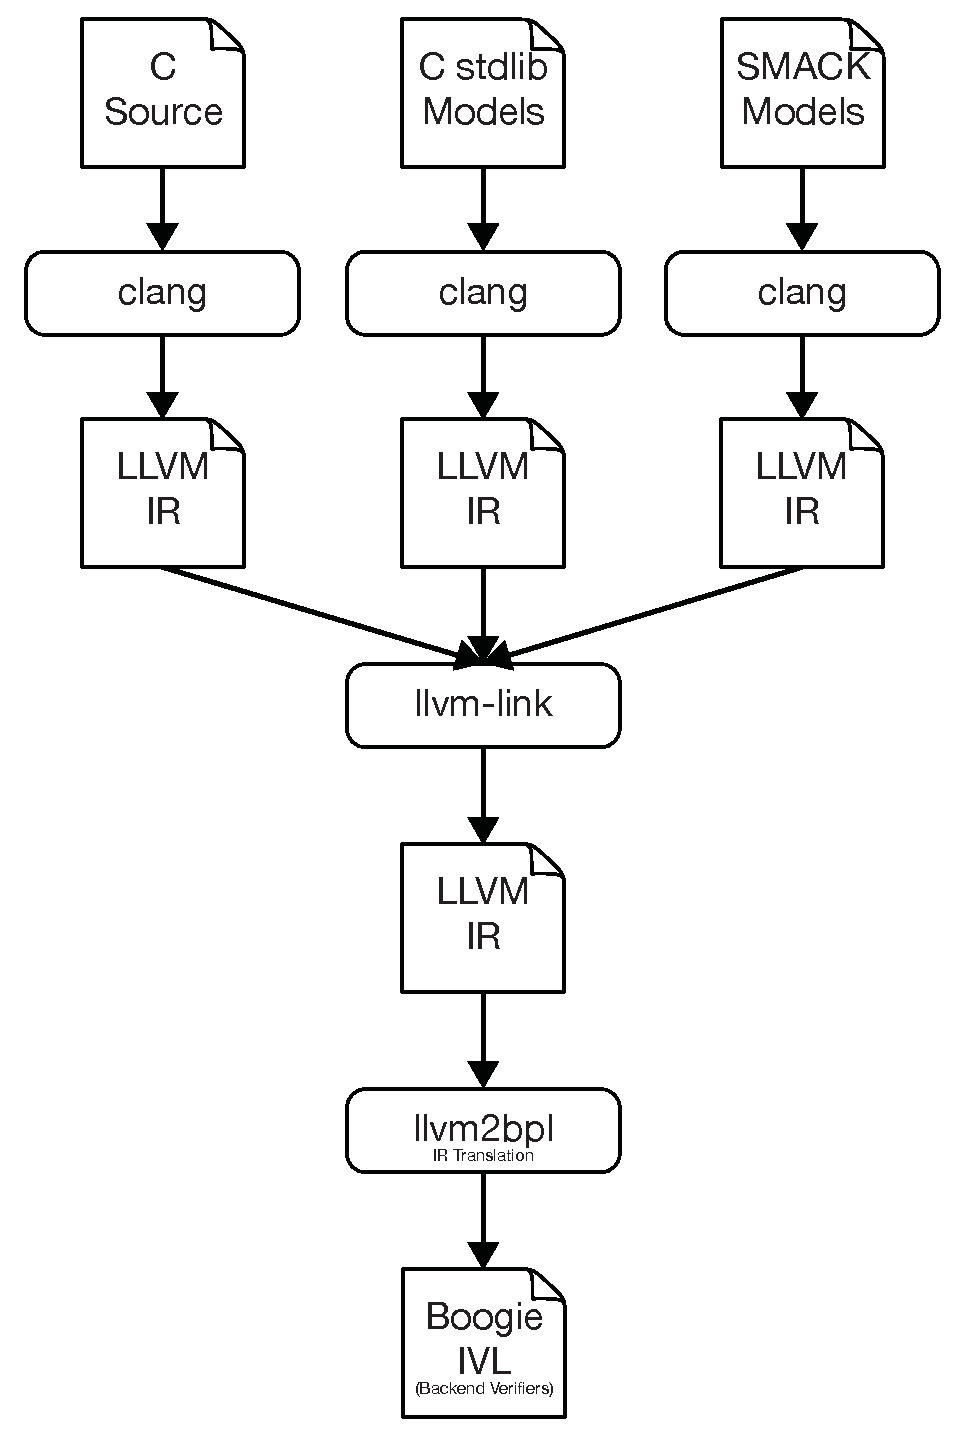
\includegraphics[width=\textwidth]{background}
% 	\caption{Toolflow of SMACK.}
% 	\label{fig:vmcaitoolflow}
% \end{figure}

% SMACK~\cite{smack-icse,smack-cav,smack-web} is an open source, modular software verification toolchain.
% %
% The core component of SMACK converts LLVM IR code into Boogie intermediate
% verification language~\cite{boogie}.
% %
% The remainder of the SMACK toolchain handles details such as compiling the
% source program into LLVM IR and invoking a Boogie verifier.
% %
% Its modular nature decouples source language details from verification by
% leveraging compiler front-ends to translate programs into the Boogie
% intermediate verification language through LLVM IR.
% %
% Before we implemented the multi-language extensions described in this chapter,
% SMACK had been predominantly used to verify LLVM IR programs produced by the
% clang C compiler.


% \cref{fig:vmcaitoolflow} shows the current toolflow of SMACK, which proceeds as
% follows:
% %
% \begin{enumerate}
% %
% \item SMACK first invokes clang, the LLVM's C compiler, to compile the input
% program, SMACK models, and C standard library models (e.g., strings, pthreads,
% math). SMACK models contain various verification primitives (e.g., for
% generating nondeterministic values) and the encoding of the memory model for
% handling of dynamically allocated memory. All of the models are written in C
% since SMACK provides a convenient mechanism for interoperating with the
% underlying Boogie code, which we describe below.
% %
% \item SMACK links together all of the generated LLVM IR files into one LLVM IR
% program.
% %
% \item The core \textsc{llvm2bpl} component of SMACK transforms an LLVM IR
% program produced by the previous step into a semantically equivalent Boogie
% program.
% %
% \item Finally, a back-end verifier, such as Corral~\cite{corral}, verifies the
% generated Boogie program using an SMT solver, such as Z3~\cite{z3}.
% %
% \end{enumerate}
% %
% In this work, we use Corral in its bounded verification mode, meaning that it
% unrolls loops and recursion up to a certain user-provided bound.


% SMACK models verifier primitives and memory models through the use of
% \lstc{\_\_SMACK\_code} function. 
% %
% This C routine takes a formatted string as a parameter, and is declared in the
% SMACK header files, but not implemented in any models. 
% %
% When \textsc{llvm2bpl} comes across a call to this function, instead of
% translating the function call, it simply inserts the parameters into the Boogie
% code snippet passed as string; this functionality is akin to C's inline
% assembly.
% %
% This allows for Boogie code or ghost variables to be injected into the
% translation, giving an easy way to encapsulate routines like \texttt{assume}
% which are not normally available in C.
% %
% It also provides an abstraction that can be used for any primitive or model.


\section{Procedure for Adding a Language}
\label{sec:procedure}

In this section, we introduce our prescribed procedure for adding support for
a new programming language into an LLVM-based software verifier.
%
The procedure is based on our study of adding languages to SMACK, but the
lessons we learned generalize to other verifiers that have similar
architecture.
%
By showing how the procedure of adding a new language to SMACK is relatively
straightforward, we also motivate the adoption of a SMACK-like verifier
architecture.
%
Note that while our procedure is focused on LLVM, we expect that a similar
process could be adopted for any IR-based verifier.
%
We structure our procedure into three tasks: interoperating with language
models, compiling into compiler intermediate representation (IR), and adding
models for missing language features.



\subsection{Interoperating with Language Models}
\label{sec:smack-code}

A software verifier has to encode the desired semantics of an input programming
language in order to perform verification.
%
In the case of an LLVM-based software verifier, that typically amounts to
providing a memory model in addition to models for LLVM IR statements generated
by the chosen compiler.
%
A memory model encodes dynamic memory allocation, pointer dereferencing, and
memory accesses.
%
Adding a new programming language necessitates for the verification to be able
to interoperate with the mentioned models.


The architecture of SMACK allows for a new programming language to easily
interoperate with SMACK models, as \cref{fig:vmcaixlang} shows.
%
First, SMACK's models for LLVM IR instructions are general and internal to
SMACK, and hence they can be shared across all languages that are compiled into
LLVM IR.
%
Second, SMACK's memory model~\cite{smack-mem-model} is encoded as a regular C
language header and its accompanying implementation.
%
This is achieved using the convenient \lstc{__SMACK_code} mechanism described
in~\cref{sec:smack-code} , which allows for the low-level model encoding to be
done at the level of C.
%
We must be able to link an input program with this header in order to
interoperate with the memory model.
%
According to our experience, most languages have interoperability with the C
language as a feature.
%
Hence, linking against the SMACK's memory model in a new programming language
is an easy task.
%
It is worth emphasizing that since the code in the new language is linking with
the C code of the memory model, every verification in a new language is already
a cross-language verification.


%To implement these verifier primitives, SMACK injects boogie code into the
%translation. It does this through the use of a special function called
%\lstc{__SMACK_code()}, which does not have a C implementation. Instead,
%whenever SMACK sees a call to \lstc{__SMACK_code()}, it hijacks the call,
%inserting the parameter (a string) into the boogie code. 
%
%
%For SMACK to verify a program in a meaningful way, the program must use
%verifier primitives like assert, assume, and nondet. SMACK implements this 
%functionality in smack.c, and exposes this in smack.h. 
%
%One limitation is that when SMACK looks for calls to \lstc{__SMACK_code()},
%it pattern-matches the function signature to the IR generated by clang's C code. 
%This means that in order to use these functions, a program must call the C functions
%defined in smack.c. In theory, \lstc{__SMACK_code()} could be re-implemented
%to pattern match the output of a different compiler, but as most languages have
%C interoperability as a feature, this is not necessary in our experience.
%
%Thus, a program to be verified must interop with SMACK's C modules, as defined
%in smack.h, to be verified properly. 


\subsection{Compiling and Linking into Compiler IR}

As opposed to verifiers that operate directly on program source, an IR-based
verifier needs for the input program to be first compiled into the chosen IR.
%
In the case of the LLVM compiler infrastructure, there are many popular
programming languages with front-ends that output LLVM IR.
%
Hence, producing LLVM IR for the programming language of choice is
typically straightforward.
%
Once the input program is compiled into IR, it gets linked with the SMACK
models, which are written in either C (common ones) or the target language
(language-specific ones) and automatically compiled by SMACK.
%
The resulting 
linked IR file is in turn handed over to the SMACK verifier for
processing (see \cref{fig:vmcaixlang}).
%
A verifier needs a program entry point, such as function \lstc{main} in C, to
know from where to start the verification process.
%
The LLVM IR specification does not prescribe a well-defined entry point, and
hence language developers are free to choose how to define the entry point for
a program in their language --- most languages define entry points other than
\lstc{main}.
%
Thus, we either implement a simple post-processing step to mark the program's
entry point, or manually specify it in SMACK's command line, which is in turn
passed to the SMACK verifier.


\subsection{Adding Models for Missing Language Features}
\label{sec:library-models}

When adding a new language, we typically observe three categories of models
that might be missing in a verifier: unsupported LLVM IR
instructions, runtime features, and standard libraries.

LLVM IR is an extensive format comprised of more than one hundred instructions
and intrinsics~\cite{llvm-lang-ref}, many of which are not commonly used.
%
Hence, when adding a new language, its compiler can potentially generate IR
instructions or intrinsics that a verifier has not encountered before, and hence are
potentially not supported.
%
This necessitates updating the verifier to account for the semantics of such
instructions.
%
Our experience shows that in the case of a mature LLVM-based verifier such as
SMACK, we rarely encountered a new compiler generating instructions/intrinsics
that it did not already support.


Most languages require the use of a standard library to achieve almost anything
of practical value.
%
SMACK provides extensive models for the C standard library, such as pthreads,
strings, and math.
%
However, every programming language comes with its own standard libraries that
it relies on, with different specifications.
%
A language may rely heavily on its standard libraries, even if it has
little or no runtime.
%
For example, unlike C, D, and Fortran, 
languages such as Rust and Swift implement arrays
as a compound type in the standard library.
%
Hence, models for the standard libraries of a new programming language have to
be written manually mostly from scratch.
%
This is the most tedious and time consuming aspect of adding support for a new
language.
%
To somewhat alleviate the burden of developing models, SMACK architecture
enables for a user to write models for standard library functions as header
files that are linked with input programs.
%
This is a convenient mechanism for writing such models since it requires no
updates to be made to the actual SMACK verifier source code.


Some languages are also heavily dependent on runtime functionality, such as
Objective-C, Swift, and Kotlin. 
%
For example, Objective-C relies heavily on its runtime for method dispatch,
memory management, and other basic features.
%
Code from the runtime is not included in the LLVM IR which is generated
by the compiler.
%
Therefore, runtime functions must be modeled before
any nontrivial verification.
%
Languages like C, Fortran, and D have very few runtime models, and as a 
result these are much easier languages to verify out-of-the-box.


\section{Case Studies}

We perform three case studies to assess the feasibility and ease of adding
support for an additional input programming language into an IR-based
software verification toolchain such as SMACK.
%
Before we describe each case study in detail, we provide our strategy for
selecting input programming languages we attempted to support.



\subsection{Choice of Input Programming Languages}



%
% how did we choose the ones we did?
%
There are numerous programming languages in existence today, and clearly it
would be infeasible for us to handle all of them.
%
Hence, for our case studies, we used the following criteria for choosing which
languages to add support for in SMACK.
%
First, we selected popular languages from the Stack Overflow Developer
Survey~\cite{devsurvey} that can be compiled down into LLVM IR.
%
Second, we performed a thorough search for other languages that can be compiled
into LLVM IR, and are important in certain domains but less popular overall
(i.e., domain specific).
%
Then, we prune this list based on our requirements on the front-end, which are
as follows:
%
\begin{enumerate}
  \item Compile input programs into LLVM IR \emph{Ahead-of-Time}
  \item Target the same version of LLVM as SMACK
  \item Be stable and under active development
\end{enumerate}
%
\cref{tab:languages} lists the languages we considered and their relevant
properties.


As SMACK directly translates an entire program from LLVM to Boogie, it requires
all related definitions to be available at translation time.
%
A \emph{Just-in-Time} compiler does not have a whole program readily
available in the LLVM IR format for SMACK to process.
%
Therefore, \emph{Ahead-of-Time} compilers are the only ones that can
currently be used with SMACK.
%
LLVM does not preserve backwards compatibility of the LLVM IR format.
%
Hence, the LLVM version supported by SMACK and the chosen language front-end
have to match.
%
The used version of SMACK supports LLVM 3.9, and hence our requirement is
for a language front-end to support the same LLVM version.
%
We sometimes had to revert to an older front-end version to satisfy this
requirement.
%
For example, Swift 4.2 does not target the required LLVM 3.9, but Swift 3.0
does.
%
Of course, as SMACK gets updated to newer LLVM versions, this requirement will
change as well.
%
In order to limit our focus to compilers of practical value, we ignore the ones
that are not stable and under active development.


Of the LLVM IR-based languages in the developer survey, there are 4 that
satisfy our criteria: C, C++, Objective-C, and Swift.
%
Kotlin, Scala~\cite{scala-link}, and C\#~\cite{llilc}) have compilers that are
not yet fully mature, but are stable and under active development.
%
We chose Kotlin as the representative of this ``managed language into LLVM IR''
category.
%
In addition to the popular languages listed on  Stack Overflow, there are other
notable, stable languages that target LLVM.
%
Most of these are tailored for domain-specific coding. 
%
The Rust programming language~\cite{rust-link} is a performant systems language
with an emphasis on safety and concurrency. 
%
The D programming language~\cite{d-link} is a mature language which offers
low-level control combined with high-level abstractions.
%
Both Rust and D target the systems programming community.
%
Fortran is primarily used in the scientific programming community, since it
provides support for parallel processing and compatibility with legacy code for
projects that span multiple decades.
%
The only language we do not use which satisfies our criteria is Haskell.
%
Its LLVM back-end is not compatible with SMACK, mainly because the entry point
for the code is not included in a standalone bitcode file.



\subsection{Case Study 1: Microbenchmarks}





We developed a microbenchmark suite to evaluate the quality of the support for
different languages we implemented in SMACK.
%
We crafted each benchmark to exercise across all languages (8 languages total,
see \cref{tab:languages}) a specific language feature we deem important,
meaning that a benchmark consists of a number of programs, each implementing
the chosen feature in a different language.
%
In addition, we injected a property to be verified into each benchmark using
assertions.
%
Hence, there are several (at least two) program versions per each
benchmark-language pair: a passing version (i.e., no failing assertions) and a
failing version (i.e., a failing assertion) for each assertion.
%
\cref{fig:microbenchmark} shows several variations of one of our
microbenchmarks.
%
\cref{tab:vmcaibenchmarks} gives basic characteristics of our microbenchmark
suite.\footnote{We made our microbenchmark suite publicly available at
\url{https://github.com/soarlab/gandalv}.}


We designed the microbenchmarks to be as small as possible, and yet still test
a particular language feature.
%
Hence, a failing benchmark is a good indicator of which feature is not properly
supported by a verifier.
%
While our microbenchmarks are not based on real-world programs, since they
focus on common and widely-used language features, being able to handle them is
a prerequisite to verifying real-world code.
%
One can think of our microbenchmarks as being \emph{litmus tests} for various
key language features.


Not all benchmarks have a program version for every language since not all
language features are supported across the board.
%
For example, languages without support for object-oriented programming (e.g.,
C, Fortran) do not have versions of the corresponding benchmark (i.e.,
method).
%
Then, Swift and Kotlin do not have syntactic support for pointers, and so we
could not implement versions of the pointer benchmark for these languages.
%
We also sometimes had to implement benchmark versions differently across
languages.
%
For example, we implemented the dynamic dispatch benchmark in Rust using
\emph{traits} instead of inheritance.
%
As another example, we implemented the inout benchmark in Swift and Fortran
using a specific mutable-parameter syntax, while in most other languages we
replicate this feature using pointers.
%
We did not implement this benchmark in Kotlin since it has no support for
pointers, nor for mutable-parameter syntax.


%Language features, such as
%for loops, may be very different across languages. In the case of for loops,
%there are a few languages (e.g. C, C++) which only use the C-style for loop,
%a few languages which only use the modern for loop (e.g. Swift), and some that
%provide both options (e.g. Objective-C). These benchmarks test the versatility
%of a verifier with respect to certain features.
%
%For SMACK, there is the added complexity of using compiled LLVM-IR. Different
%langauges compile, say, for loops in different ways. For example, Kotlin and
%Swift both use range objects to compile for loops. However, Kotlin compiles it's
%range object into LLVM, while Swift uses a standard library class. 





\cref{tab:results} summarizes the results of running SMACK with our
extensions on the microbenchmarks.
%
Overall, SMACK successfully discharges all available program versions of
benchmarks in C, Fortran, and Rust.
%
For C++ and D, the main missing language feature that we still have to add
support for is dynamic dispatch.
%
Swift, Objective-C, and Kotlin need more work before SMACK could support
language features beyond just the very basic ones.
%
The primary cause for the failing benchmarks is SMACK lacking models of
standard libraries and runtime.


Swift, Objective-C, Kotlin, and Rust are all very library- and
runtime-depen\-dent.
%
Hence, there are many basic language features that SMACK does not capture
precisely (i.e., that are not modeled in SMACK), which causes even some small
benchmarks to fail.
%
As we note in \cref{sec:large-runtimes}, developing such models for a
verifier is typically a tedious manual process, and is an exercise we could not
perform for all languages in the limited amount of time we had for our case
study.
%
%In our previous work~\cite{atva-paper}, we describe our experience of
%implementing models of several popular Rust standard library functions, which
%we used in this work as well.
However, the version of SMACK we used already contained models
of several popular Rust standard library functions.
%
Hence, in our experiments, the other three languages have more failing
benchmarks than Rust, which are caused by the following unmodeled
functionality:
%
\begin{itemize}
  \item \textbf{Swift} range structures (forloop), array subscripts (array), dispatching functions via function pointers (method)
  \item \textbf{Obj-C} objc-msg-send for dispatching methods via function pointers (compound, method), NSArray class (array)
  \item \textbf{Kotlin} dynamic object instantiation (compound, array)
\end{itemize}
		
%\subsubsection{Vtables}
%
%SMACK currently does not support the use of Vtables for dynamic dispatch. Because
%of this, it cannot tell between different overrides of the same method in
%different classes. Every language which supports objects and inheritence thus
%fails the dynamic benchmark. 
%
%However, Rust uses a different method to accomplish dynamic dispatch, so its
%benchmark is properly supported.


\subsection{Case Study 2: Adding a Language}



In order to get a rough estimate of the time commitment required to add support
for a new language to an IR-based verifier, we conducted an informal timed
exercise where an undergraduate student working on this project (Jack
J.~Garzella, one of the coauthors) added support for one additional language,
the D programming language, to SMACK.
%
During the exercise, the student followed the steps we prescribe in our procedure from
\cref{sec:procedure}, and we measured elapsed time (in hours) it took him
to accomplish each of the steps.
%
\cref{tab:d-exercise} summarizes our measurements.


The student had no experience with D beyond implementing the microbenchmarks;
he was also not familiar with the SMACK internals, which ended up not being
important for this exercise since no changes to SMACK were needed.
%
However, as D was the sixth programming language the student added, he had
ample experience adding support for new languages, which contributed to this
exercise proceeding smoothly.
%
Furthermore, D was an easy language to add since the LLVM IR it generates is
close to the one generated by the C clang compiler, and hence heavily tested
with SMACK.
%
In addition, basic code in D does not heavily depend on its standard library
and runtime.
%
Hence, the student spent very little time modeling missing functions for D.
%
For languages with extensive usage of standard libraries and runtime (e.g.,
Swift, Kotlin), we expect that modeling the runtime and standard library
functionality to dominate the total time.



\subsection{Case Study 3: Cross-Language Verification}

%\begin{lstlisting}[language=C,basicstyle=\ttfamily\scriptsize, commentstyle=\color{green},frame=lines,numberstyle=\tiny]
%void order(int * a, int *b, int *c) {
%  if (*a > *b) {
%    int tmp = *a;
%    *a = *b;
%    *b = tmp;
%  }
%  if (*b > *c) {
%    int tmp = *b;
%    *b = *c;
%    *c = tmp;
%  }
%  if (*a > *b) {
%    int tmp = *a;
%    *a = *b;
%    *b = tmp;
%  }
%}
%
%int classify_triangle_sides_c(int s1, int s2, int s3) {
%  int *a = &s1;
%  int *b = &s2;
%  int *c = &s3;
%
%  order(a,b,c);
%
%  if (*a == *b && *b == *c) { // equilateral
%    return 0;
%  } else if (*a == *b || *b == *c) { // iscoseles
%    return 1;
%  } else { // scalene
%    return 2;
%  }
%}
%\end{lstlisting}

One of the major advantages to the IR-based approach to verification is the
ease of cross-language verification. 
%
In fact, with the approach that SMACK takes, every verification (of a non-C
language) is a cross-language verification, as SMACK's models that have to be
linked against the input program are written in C.
%
With this in mind, non-trivial cross-language verification efforts are
typically as simple as any regular single-language verification.
%
As a proof of this concept, we took a simple algorithm, namely a classic
triangle classifier, and implemented it in C, Rust, and Fortran.
%
Our triangle classifier takes 3 integers as input, which represent the sides of
a triangle, and it determines and returns the type of the triangle defined by
the input sides.
%
We wrote a harness program that invokes triangle classifiers from
each language in turn, feeds equal nondeterministic inputs to all of them, and
asserts that they return the same result.
%
Hence, we performed cross-language verification to verify the equivalence of
our implementations in all three languages.
%
SMACK was able to verify the equivalence (i.e., the harness program) in around
19 seconds.
%
We expect such cross-language equivalence checking to be a valuable tool for
developers when rewriting legacy applications in, for example Fortran or C,
into more modern languages, such as C++ or Rust.


% \begin{table}[tb]
% \caption[Equivalence checking of half-precision floating-point
%   implementations in C and Rust]{Equivalence checking of half-precision floating-point
%   implementations in C and Rust.
%   % 
% %  Column \textbf{Function} shows the methods of Rust \textit{f16} type.
%   %
%   Column \textbf{Equal?} shows whether the two implementations
%   are equivalent;
%   %
%   column \textbf{Time} gives the verification runtime in seconds;
%   %
%   column \textbf{LOC} gives the number of lines of code in the checked Rust function.
%   }
%   \label{tab:rust-half}
% \centering
% \vspace{1em}
% \setlength{\tabcolsep}{8pt}
% \ra{1.75}
% \begin{tabular}{@{}lcrr@{}}
% \toprule
% \textbf{Function} & \textbf{Equal?} & \textbf{Time(s)} & \textbf{LOC} \\
% \midrule
%   eq        & \cmark{} & 13 & 8 \\
%   lt        & \cmark{} & 22 & 13 \\
%   le        & \cmark{} & 18 & 13 \\
%   gt        & \cmark{} & 17 & 13 \\
%   ge        & \cmark{} & 18 & 13 \\
% \hdashline[1pt/1pt]
%   to\_f32   & \cmark{} & 8  & 41 \\
%   to\_f64   & \cmark{} & 8 & 41 \\
%   from\_f32 & \xmark{} & 5 & 68 \\
%   from\_f64 & \xmark{} & 4 & 70 \\
% \hdashline[1pt/1pt]
%   is\_nan   & \cmark{} & 4 & 3\\
% \bottomrule
% \end{tabular}
% \end{table}


We further push our cross-language verification case study to a real-world Rust
application --- the \textit{half} crate~\cite{rust-half} that implements the
half-precision floating-point type \lstrust{f16}.
%
We chose the \textit{half} crate because its implementation is compact in terms
of code size (functions range from only a few to around 70 LOC, see
\cref{tab:rust-half}), but difficult to reason about because it frequently
performs low-level bit manipulations. 
%
Furthermore, the equivalence of functions implementing the half-precision
floating-point type can be easily expressed.
%
This makes the \textit{half} crate a suitable target for our cross-language
verification case study.


For the purpose of this case study, we developed a simple C reference
implementation of the half-precision floating-point type that leverages the
available \lstc{__f16} type.
%
Then, we verify that several important representative methods of the
\textit{half} crate, such as \lstrust{lt}, \lstrust{gt}, and \lstrust{to\_f32},
are equivalent to the respective C implementations.
%
We leverage the Rust's \emph{Foreign Function Interface} to write harness
programs that assert the equivalence between Rust and C functions.
%
(Note that if such a mechanism for interoperating between languages does not
exist, we could implement the equivalence check at the LLVM IR level; however,
working directly with the low-level LLVM IR would be more tedious.)
%
Thanks to Rust's high interoperability with C, we are able to trivially express
equivalence using the equality operator.
%
For example, relational operators in C evaluate to 1 if the relation is true
and otherwise they evaluate to 0.
%
In Rust, casting a value of type \lstrust{bool} into an integer has the same
behavior.
%
Therefore, comparing a predicate function such as \lstrust{eq} in C and Rust
reduces to checking if the return value of the C version is equal to the return
value of the Rust version cast to type \lstrust{u8}.



\cref{tab:rust-half} summarizes the results of this case study.
%
SMACK is able to verify that most of the chosen functions of the \lstrust{f16}
type are equivalent to their reference C implementations.
%
The only exceptions are functions from\_f32 and from\_f64, for which SMACK
discovered inconsistencies between the two implementations: conversions from
larger bit-width floating-point types to \lstrust{f16} are rounded differently.
%
We reported this issue to the \textit{half} crate developers, and they
confirmed and fixed it.
%
The verification runtimes range between 4--22 seconds on a 3.5GHz Intel 3770k
machine.


\section{Experience}
\label{sec:experience}

In this section, we describe our experience of applying the procedure
introduced in \cref{sec:procedure} to add support for new languages
into SMACK as well as perform cross-language verification.
%
First, we discuss why our approach and procedure allow us to trivially
support many language constructs of the added programming languages
(\cref{sec:supported-features}).
%
Second, we describe key challenges that we encountered in the process of
adding support for new languages and propose solutions for them
(\cref{sec:challenges-solutions}).
%
Third, we present our experience with leveraging the cross-language verification
capability to perform equivalence checking (\cref{sec:cross-language}).



\subsection{Trivially Supported Features}
\label{sec:supported-features}

SMACK is a mature C verifier that has been successfully applied on numerous
C programs, including large-scale real-world C projects such as OpenSSH, SQLite,
and Linux device drivers.
%
Hence, SMACK already fully supports an extensive subset of LLVM IR that gets
generated by the clang C compiler.
%
For example, the key language constructs of LLVM IR such as functions, control
flow, arithmetic, and derived types are completely modeled.
%
As a result, SMACK readily supports new languages of which compilers emit LLVM
IR code that is akin to what clang generates.
%
We find that these languages are typically also procedural C-like languages,
such as Fortran and D.


As it turns out, to our surprise, SMACK was often able to out-of-the-box
support even language features that are not found in C.
%
For example, without any modifications SMACK could handle the vectorized
addition of arrays in Fortran, which we show in \cref{fig:fortran-ex}.
%
After inspecting the IR code generated by the Fortran compiler, we observe that
the vectorized addition operation compiles into an element-wise array addition,
which is a common IR operation and hence was already supported by SMACK.

%Modifications, while trivial, are still required. For example, LLVM IR allows
%arbitrary characters to compose identifier names.
%
%However, Boogie identifier names are much more restricted which only allow
%alphanumeric characters plus a limited set of special characters.
%
%Both Objective-C and Kotlin make use of semicolons in their LLVM names and Kotlin
%even uses semicolons, angle brackets, and parenthesis.
%
%Simply translating these identifiers to identical Boogie
%identifiers as what is done in the C support causes syntax errors.
%
%However, A simple extension to SMACK's naming policies easily fixes this problem.

Having an extensive subset of LLVM IR supported also saved us from modeling a
lot of key program constructs in non-C-like languages such as Rust and Swift.
%
For example, even though function calls and control flow constructs are
different from those found in C (e.g., closures and match expressions), they
are compiled to the subset of LLVM IR that was already understood by SMACK.
%
Therefore, our approach enables us to evade cumbersome modeling of advanced
language features such as closures.
%
In this regard, our experience demonstrates the advantages of our IR-based
approach for multi-language verification.


%\subsection{Runtime Sizes}
%
%We define the \textit{runtime} of a programming langauge to be all functionality
%that is 1) necessary for a user to write real code, and 2) is not written by the
%user. For example, the C runtime includes methods such as \lstc{malloc},
%\lstc{free}, and string processing methods like \lstc{strlen}.
%
%In the context of LLVM, runtime functions and datatypes are often declared but
%not implemented in compiled IR, with the expectation that runtime code will be
%linked in before runtime. As a translator, SMACK does not have access to these
%implementations. Therefore, any runtime functionality must be modeled by SMACK.
%
%As a general rule, the time it takes to add robust support for a langauge to
%SMACK is directly proportional to the size of its runtime. For example, C
%has a very small runtime and is easily supported, and Objective-C has an
%extensive runtime and take quite a bit of work to support.
%
%As such, we divide all of our suitable LLVM compilers into two categories:
%those with a small runtime, those with an extensive runtime, and those
%whose compilers are not suitable for SMACK.
%
%\textbf{Small Runtime}
%\begin{itemize}
%    \item C (clang)
%    \item C++ (clang)
%    \item D (ldc)
%    \item Fortran (flang)
%\end{itemize}
%
%\textbf{Large Runtime}
%\begin{itemize}
%    \item Objective-C (clang)
%    \item Rust (rustc)
%    \item Swift (swiftc)
%    \item Kotlin (kotlinc)
%\end{itemize}
%
%\subsection{Languages with a Small Runtime}
%
%Each of these languages required small changes to SMACK and it's tooling
%to support, but there were no modifications that went beyond the level of
%a bugfix or small enhancement.
%Fortran is of particular note among these languages because it did not require
%any internal modifications to SMACK at all.
%
%An example of such a problem is escaping more characters in names. LLVM IR allows
%arbitrary characters to be in identifier names. However, boogie identifiers are
%much more restricted and only allow alphanumeric characters plus a limited set
%of special characters. For example, colons and semicolons are not allowed in
%boogie identifiers, but can be used in LLVM identifiers. Clang's C support does
%not use this functionality, but other langauges often do. Before this was fixed,
%SMACK would simply copy the boogie-invalid LLVM identifier, causing crashes.
%A simple extension to SMACK's internal naming class fixed this problem.
%
%Despite being similar to C, all of the languages with small runtimes
%have features that C itself does
%not support.
%Thus, there are many features that C does not have, which
%SMACK is able to support out of the box. This is the power of targeting LLVM.
%
%One example of a SMACK-supported non-C
%feature is class declarations with fields.
%In D, we can define a class such as:
%
%\begin{lstlisting}
%class Point
%{
%    int x;
%    int y;
%    this(int _x, int _y) {
%        x = _x;
%        y = _y;
%    }
%}
%\end{lstlisting}
%
%When this is compiled into LLVM, it becomes a struct type:
%
%\begin{lstlisting}
%%compound.Location = type { %compound.Location.__vtbl*, i8*, i32, i32 }
%\end{lstlisting}
%
%Methods are compiled into LLVM procedures, like any C function.
%
%Array in Fortran are compiled into pointers, so that once they are
%compiled, they look similar to compiled C arrays. Consider the following
%start of a subroutine declaration (free-form Fortran is used for readibility):
%
%\begin{lstlisting}
%subroutine process_vectors(A,B,S)
%  implicit none
%  integer, dimension(2) :: A, B, S
%\end{lstlisting}
%
%The above declaration is translated into the following
%llvm declaration:
%
%\begin{lstlisting}
%define internal void @process_vectors_(i64* %a, i64* %b, i64* %s) #0 !dbg !59 {
%\end{lstlisting}
%
%We can see that the parameters, A, B, and S, all of which are integer arrays of
%length 2 based on the declaration, compile into pointers to integers in LLVM IR.


\subsection{Adding New Languages: Challenges and Solutions}
\label{sec:challenges-solutions}

As expected, supporting even a small subset of a new language in a verifier
is often challenging.
%
For example, a major challenge is the need to model previously unsupported LLVM
IR constructs.
%
Our experience shows that the compilers of non-C-like languages, such as Rust
and Swift, indeed produce LLVM IR that was not supported by SMACK.
%
Moreover, another important challenge is that we have to model a language
runtime and its standard libraries to enable for practically usable
verification.
%
In the rest of this section, we describe in detail these challenges as well as
our efforts to solve them.


\subsubsection{Unsupported LLVM Constructs}

SMACK is a mature verifier that has been thoroughly tested on C programs,
including thousands of SVCOMP benchmarks as well as large real-world
applications such as OpenSSH.
%
Despite SMACK's maturity, we found that compilers for the emerging languages,
such as Rust and Swift, readily generate LLVM IR constructs we do not observe in
LLVM IR generated from C code by clang.
%
Hence, we had to extend SMACK with support for such constructs, and we
describe some of these next.


%
% handling of structures
%
Both the Rust and Swift compilers heavily rely on the use of LLVM structure
types, often emitting different instructions involving structures than what
clang would generate.
%
We solved this problem by modeling LLVM IR structure types using
uninterpreted functions that recursively constrain each
field.
%
For example, we represent value \lstllvm{\{v,1\}} of structure type \lstllvm{\{T,i1\}}
using an integer \lstboogie{s} with constraint
\lstboogie{f(s,0)==v && f(s,1)==1}, where \lstboogie{f} is an
uninterpreted function with the second argument being the index of a
structure field.
%
This encoding allows us to model two basic LLVM IR structure instructions
\lstllvm{extractvalue} and \lstllvm{insertvalue} that read and write
structure fields, respectively.
%
Loads and stores of structures into memory are recursively translated into a
sequence of instructions that generate load/store for each field of
primitive type, in conjunction with the two aforementioned instructions.

Another previously unsupported but frequently used LLVM IR construct is intrinsics.
%
% summarize integer overflow intrinsics
%
For example, both the Rust and Swift compilers default to using LLVM IR's
overflow arithmetic intrinsics, such as
\lstllvm{llvm.add.with.overflow.i32}.
%
The \lstrust{leading_zeros} methods of unsigned integer types in Rust are
compiled to \lstllvm{llvm.ctlz.*} intrinsics.
%
Such intrinsics can be easily modeled.
%
For example, we model these intrinsics in SMACK by first performing the
requested operation in the double-bit-width precision, to avoid potential
overflows.
%
Then, we inspect the result to detect if it overflowed, in which case we either
report an overflow error or we block the overflowing path.


In addition to supporting more LLVM IR instructions, we also extended SMACK
to support instruction sequences that are not regularly generated by clang.
%
For example, the Rust compiler performs a \emph{packing} optimization where
structures with a size less than 8 bytes are packed into 8 byte integers
(e.g., a load of a structure of type \lstllvm{\{i32,i32\}} gets encoded as a
load of \lstllvm{i64}).
%
This breaks the completeness of SMACK's memory model~\cite{smack-mem-model},
which is not precise enough to capture such low-level operations, thereby
leading to false alarms.
%
We added an analysis pass to SMACK that detects load/store instruction
patterns with pointer operands of integer element type that refer to
structures.
%
We translate such patterns to load from or store into structure fields
(following the encoding described earlier), thereby avoiding packing.

Although we had to model these additional constructs, our approach still
demonstrates the advantages discussed in \cref{sec:supported-features}:
%
modeling one LLVM IR construct benefits the support of multiple languages,
and this process becomes progressively easier as adding a new language
benefits from previous modeling efforts.


\subsubsection{Languages with Large Runtimes}
\label{sec:large-runtimes}

Getting a verifier to translate LLVM IR generated from a language with a
large runtime is not any more difficult than for languages with smaller
runtimes.
%
However, performing a nontrivial verification task for such a language is
much harder, because even rudimentary language features are sometimes under
the hood implemented using complex runtime constructs and standard
libraries.
%
Moreover, the source code implementing such features is not
readily accessible to the verifier as IR code linked with the program
source.
%
We found this to be the most challenging problem when adding a new language
to a verifier.
%
Note that this problem persists even if the verification is done directly on
program source (as opposed to IR) since the source code of the underlying
runtime is typically not available, written in a different programming
language, or too large to be efficiently handled by a verifier.


As an example of such a language feature, consider the for-in loop over an
iterable structure.
%
All of the languages with substantial runtime we considered provide such a
feature.
%
In fact, in Swift, Kotlin, and Rust, the C-style for loop is not even
supported, and range structures are used to emulate the same behavior.
%
Consider this simple example in Swift:
\lstswift{for i in 0..<10 \{x += 5\}}.
%
The compiler translates the code \lstswift{0..<10} using a
\lstswift{Range<Int>} structure/class, whose member methods are then called
in the compiled loop code.
%
The code of such member methods is not readily available to the verifier,
but is a part of the runtime.
%
On the other hand, both Kotlin and Rust compile such loops into basic LLVM
IR instructions that do not contain method calls into runtime, despite the
high-level concept of a range being similar to Swift. 
%
Many features of large-runtime languages are implemented like this, and they
vary wildly between languages. 
%
Examples of other basic language features the heavily depend on runtime
include method dispatch (Swift, Objective-C), arrays (Swift, Objective-C,
Rust, Kotlin), and object instantiation (Kotlin).
%
As a more extreme example, even basic arithmetic in Kotlin is abstracted
into invoking methods belonging to its runtime, instead of generating the
appropriate LLVM IR instructions directly.
%
We relied on two solutions to overcome such problems, with different
trade-offs, as we describe next.


We compile and link an existing implementation of the runtime/standard
library with the input program.
%
For example, to support basic integer operations in Kotlin, we used the
existing implementation of these operations from the Kotlin runtime and
linked it with the input program. 
%
The main advantage of this approach is that it requires no manual effort.
%
It also avoids the user potentially introducing errors while modeling the
runtime.
%
The main drawback is that the standard libraries and runtime are generally
very large, and this may cause verification to blow up even on small input
programs. 
%
For example, the implementation of the array structure in Swift is thousands
of lines of code.
%
Such code is also heavily optimized, and often relies on low-level bit
vector operations and compiler builtins, which further complicate its
verification.

% \begin{table}[p]
% \caption[Sizes of models we developed for each language]{Sizes of models we developed for each language.
%   Column \textbf{Model LOC} gives the size of each model
%   in terms of lines of code.
% }
% \label{tab:model-sizes}
% \vspace{1em}
% \centering
% \setlength{\tabcolsep}{8pt}
% \ra{1.75}
% \begin{tabular}{@{}lr@{}}
% 	\toprule
% 	\textbf{Language} & \textbf{Model LOC} \\
% 	\midrule
% 	C &  2566 \\
% 	C++ &  13 \\
% 	Fortran &  38 \\
% 	D &  0 \\
% 	Rust & 480 \\
% 	Objective-C & 0 \\
% 	Swift &  2 \\
% 	Kotlin & 17 \\
% 	\bottomrule
% \end{tabular}
% %\vspace{-3mm}
% \end{table}


We model the standard libraries and runtime by writing stubs for the
relevant methods.
%
\cref{tab:model-sizes} gives the sizes of the models we developed for each
language we support.
%
SMACK already came with extensive models for the C standard library and a part
of the Rust standard library, which is why these two models are by far the
largest.
%
The main advantage of this approach is that the manually written models make
the verification much more tractable, and hence most verifiers, no matter
whether they are IR-based or not, require it to achieve scalable verification.
%
The main drawback is that writing them is a tedious manual effort that
requires detailed understanding of the language specifications.
%
Hence, we did not do that for other languages.
%
In principle, the standard libraries and runtime of Kotlin, Objective-C, and
Swift could each be modeled in a similar way to Rust.
%
Note that this solution is contradictory to the general principle of our
approach since it requires per-language modeling.


\subsection{Cross-Language Verification}
\label{sec:cross-language}
%
Although our experience with cross-language verification is limited to
equivalence checking of programs written in different languages, it captures an
important pattern in cross-language development: a program written in one
language uses external libraries written in another language.
%
Furthermore, equivalence checking is a useful application of cross-language
verification, giving confidence to developers that a new, native implementation
of a library retains the behaviors of the previous non-native implementation.
%
This is especially true when large rewriting efforts are under way, such as
replacing legacy libraries implemented using Fortran with C/C++ implementations
in the context of high-performance computing, or libraries implemented using C
with their Rust counterparts.


We find that once the languages involved in the cross-language verification
process are well-supported and there are available mechanisms for these
languages to interoperate, cross-language verification is feasible, highly
automated, and comes almost for free.
%
This is expected since our approach casts the problem of cross-language
verification into the problem of verifying a single language, namely LLVM IR.
%
Therefore, the main impediments we encountered while verifying cross-language
programs were related to SMACK's incomplete support for LLVM IR, similarly to
our efforts to add support for new languages.
%
For example, while performing the case study, the only issue we encountered was
that SMACK did not model the LLVM count-leading-zeros intrinsics.
%
We quickly added support for this instruction and were able to complete the
verification process smoothly.

\section{Conclusions}
\label{sec:conclusions}

In this chapter, we proposed a procedure for extending an IR-based verifier
with multi- and cross-language verification capabilities.
%
By relying on the proposed procedure, we extended the LLVM IR-based SMACK
software verification tool\-chain with basic prototypical support for 6
additional languages.
%
We performed several case studies to assess the quality of our extensions and
the feasibility of leveraging the IR-based verifier architecture in the context
of multi- and cross-language verification.
%
Our evaluation is encouraging and indicates that the IR-based architecture
indeed lowers the bar for adding support for a new language into an existing
verifier --- languages with small runtimes could be reliably added with only a
modest effort.
%
It also allows for straightforward cross-language verification.
%
As we anticipated, supporting languages with large runtimes that heavily rely
on standard libraries is possible, but mature support would require a large
manual effort to model the runtime and libraries.

% \begin{figure}[tb]
% 	\centering
% 	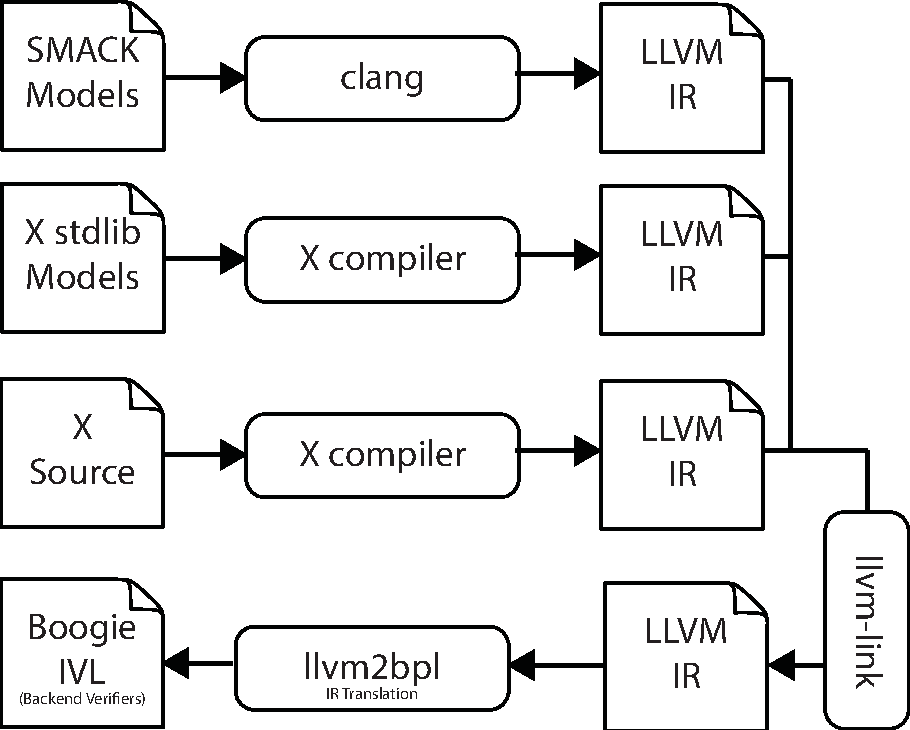
\includegraphics[width=\textwidth]{procedure}
% 	\caption{Toolflow for adding support for programming language X to SMACK.}
% 	\label{fig:vmcaixlang}
% \end{figure}

% \begin{table}[tb]
% \caption[List of programming languages we considered and their properties]{List of programming languages we considered and their properties.
%   Column \textbf{Ahead-of-Time} shows whether an Ahead-of-Time compiler
%   is available for the language;
%   %
%   column \textbf{LLVM 3.9} indicates whether the needed LLVM version is
%   supported;
%   %
%   column \textbf{Active} indicates whether the compiler is under active
%   development, while column \textbf{Stable} indicates if there is a
%   stable release;
%   %
%   and finally, column \textbf{Used it?} shows whether we used the language
%   in our evaluation.

% }
% \label{tab:languages}
% \centering
% \setlength{\tabcolsep}{6.5pt}
% \ra{2}
% \vspace{1em}
% \begin{tabular}{@{}lcccccc@{}}
% 	\toprule
% 	\textbf{Language} & \textbf{Compiler} & \textbf{Ahead-of-Time} & \textbf{LLVM 3.9} & \textbf{Active} & \textbf{Stable} & \textbf{Used it?} \\
% 	\midrule
% 	C & clang & \cmark & \cmark & \cmark & \cmark & \cmark \\
%         \hdashline[1pt/1pt]
% 	C++ & clang & \cmark & \cmark & \cmark & \cmark & \cmark \\
%         \hdashline[1pt/1pt]
% 	Fortran~\cite{flang-link} & flang & \cmark & \cmark & \cmark & \cmark & \cmark \\
%         \hdashline[1pt/1pt]
% 	D~\cite{d-link} & ldc & \cmark & \cmark & \cmark & \cmark & \cmark \\
%         \hdashline[1pt/1pt]
% 	Rust~\cite{rust-link} & rustc & \cmark & \cmark & \cmark & \cmark & \cmark \\
%         \hdashline[1pt/1pt]
% 	Objective-C & clang & \cmark & \cmark & \cmark & \cmark & \cmark \\
%         \hdashline[1pt/1pt]
% 	Swift~\cite{swift-link} & swiftc & \cmark & \cmark & \cmark & \cmark & \cmark \\
%         \hdashline[1pt/1pt]
% 	Kotlin~\cite{kotlin-link} & kotlinc & \cmark & \cmark & \cmark & \cmark & \cmark \\
%         \hdashline[1pt/1pt]
% 	Scala~\cite{scala-link} & scala-native & \cmark & \cmark & \cmark & \cmark & \xmark \\
%         \hdashline[1pt/1pt]
% 	C\#~\cite{llilc} & llilc & \cmark & ? & \cmark & \cmark & \xmark \\
%         \hdashline[1pt/1pt]
% 	Haskell~\cite{haskell-link} & ghc & \cmark & \cmark & \cmark & \cmark & \xmark \\
%         \hdashline[1pt/1pt]
% 	Julia~\cite{julia} & julia & \xmark & \cmark & \cmark & \xmark & \xmark \\
%         \hdashline[1pt/1pt]
% 	Go~\cite{go-link} & llgo & \cmark & \cmark & \xmark & \xmark & \xmark \\
%         \hdashline[1pt/1pt]
% 	Python~\cite{pyston-link} & pyston & \cmark & ? & \xmark & \xmark & \xmark \\
%         \hdashline[1pt/1pt]
% 	Ruby~\cite{ruby-link} & ruby-llvm & \cmark & \xmark & \xmark & \xmark & \xmark \\
%         \hdashline[1pt/1pt]
% 	Java~\cite{falcon-link} & falcon (Azul) & \xmark & \xmark & \cmark & \xmark & \xmark \\
% 	\bottomrule
% \end{tabular}
% \end{table}


% \begin{figure}[tb]
% 	\centering
% 	\begin{minipage}{.45\textwidth}
% \begin{lstlisting}[language=C,basicstyle=\ttfamily\large,commentstyle=\color{green},frame=lines,numberstyle=\tiny]
% int cap(int x) {
%   int y = x;
%   if (10 < x) {
%     y = 10;
%   }
%   return y;
% }

% int main(void) {
%   assert(cap(2)==2);
%   assert(cap(15)==10);
%   int x = nondet_int(); 
%   assert(cap(x) <= 10);
% }
% \end{lstlisting}
% 	\end{minipage}
% \hfill
% 	\begin{minipage}{.5\textwidth}
% \begin{lstlisting}[language=swift,basicstyle=\ttfamily\large,commentstyle=\color{green},frame=lines,numberstyle=\tiny]
% func cap(_ x: Int)->Int
% {
%   var y = x
%   if 10 < x {
%     y = 10
%   }
%   return y
% }

% assert(cap(2) == 2)
% assert(cap(15) == 10)
% let x=Int(nondet_int())
% assert(cap(x) <= 10)
% \end{lstlisting}    
%     \end{minipage}
% 	\begin{minipage}{.45\textwidth}
% \begin{lstlisting}[language=rust,basicstyle=\ttfamily\large,commentstyle=\color{green},frame=lines,numberstyle=\tiny]
% fn cap(x: usize)->usize
% {
%   let mut y = x;
%   if 10 < x {
%     y = 10;
%   }
%   return y;
% }


% fn main() {
%   let two = cap(2);
%   let ten = cap(15);
%   assert!(two == 2);
%   assert!(ten == 10);
%   let x = nondet_int();
%   assert!(x <= 10);
% }
% \end{lstlisting}
% 	\end{minipage}
% \hfill
% 	\begin{minipage}{.5\textwidth}
% \begin{lstlisting}[language=fortran,basicstyle=\ttfamily\large,commentstyle=\color{green},frame=lines,numberstyle=\tiny]
% pure function cap(x)
%  integer, intent(in)::x
%  integer :: cap, y
%  y = x
%  if (10 < y) then
%    y = 10
%  end if
%  cap = y
% end function

% program main
%  integer :: cap, x
%  call assert(cap(2)==2)
%  call assert(cap(15)==10)
%  x = nondet_int()
%  call assert(cap(x)<=10)
% end program main
% \end{lstlisting}    
%     \end{minipage}
% \caption{Microbenchmark with program versions in C, Swift, Rust, and Fortran.}
% \label{fig:microbenchmark}
% \end{figure}


% \begin{table}[tb]
% \caption[Characteristics of our microbenchmark suite]{Characteristics of our microbenchmark suite. Column \textbf{LOC} is the average
% number of lines of code per benchmark across supporting languages; column \textbf{\#Lang}
% is the number of languages supporting the features tested.}
% \vspace{1em}
% \label{tab:vmcaibenchmarks}
% \centering
% \setlength{\tabcolsep}{20pt}
% \ra{1.75}
% 	\begin{tabular}{@{}lcrr@{}}
% 	\toprule
% 	\textbf{Benchmark} & \textbf{Features Tested} & \textbf{LOC} & \textbf{\#Lang} \\
% 	\midrule
% 	basic    & basic assertions & 8 & 8 \\
%         \hdashline[1pt/1pt]
% 	compute  & integer arithmetic & 12 & 8 \\
%         \hdashline[1pt/1pt]
% 	function & functions, if-then-else, nondet values & 19 & 8 \\
%         \hdashline[1pt/1pt]
% 	forloop  & for loops & 14 & 8 \\
%         \hdashline[1pt/1pt]
% 	fib      & recursion & 20 & 8 \\
%         \hdashline[1pt/1pt]
% 	compound & objects and structures, fields & 18 & 8 \\
%         \hdashline[1pt/1pt]
% 	array    & array creation, array access & 10 & 8 \\
%         \hdashline[1pt/1pt]
% 	pointer  & dynamic memory allocation, references & 14 & 6 \\
%         \hdashline[1pt/1pt]
% 	inout    & updates via side effects & 17 & 7 \\
%         \hdashline[1pt/1pt]
% 	method   & single type dispatch & 26 & 6 \\
%         \hdashline[1pt/1pt]
% 	dynamic  & polymorphic dispatch & 29 & 6 \\
% 	\bottomrule
% \end{tabular}
% \end{table}

% \begin{table}[tb]
% \caption[Results of running SMACK on our microbenchmarks]{Results of running SMACK on our microbenchmarks. Symbol \cmark marks
% passing, symbol \xmark failing, and \notapplic marks benchmarks that do
% not have a version for the corresponding language.}
% \label{tab:results}
% \centering
% \setlength{\tabcolsep}{9pt}
% \vspace{1em}
% \ra{2}
% \begin{tabular}{@{}lcccccccc@{}}
% \toprule
% \textbf{Benchmark} & \textbf{C} & \textbf{C++} & \textbf{Objective-C} & \textbf{Rust} & \textbf{Fortran} & \textbf{D} & \textbf{Swift} & \textbf{Kotlin} \\
% \midrule
% basic & \cmark & \cmark & \cmark & \cmark & \cmark & \cmark & \cmark & \cmark \\
% \hdashline[1pt/1pt]
% compute & \cmark & \cmark & \cmark & \cmark & \cmark & \cmark & \cmark & \cmark \\
% \hdashline[1pt/1pt]
% function & \cmark & \cmark & \cmark & \cmark & \cmark & \cmark & \cmark & \cmark \\
% \hdashline[1pt/1pt]
% forloop & \cmark & \cmark & \cmark & \cmark & \cmark & \cmark & \xmark & \cmark \\
% \hdashline[1pt/1pt]
% fib & \cmark & \cmark & \cmark & \cmark & \cmark & \cmark & \cmark & \cmark \\
% \hdashline[1pt/1pt]
% compound & \cmark & \cmark & \xmark & \cmark & \cmark & \cmark & \cmark & \xmark \\
% \hdashline[1pt/1pt]
% array & \cmark & \cmark & \xmark & \cmark & \cmark & \cmark & \xmark & \xmark \\
% \hdashline[1pt/1pt]
% pointer & \cmark & \cmark & \cmark & \cmark & \cmark & \cmark & \notapplic & \notapplic \\
% \hdashline[1pt/1pt]
% inout & \cmark & \cmark & \cmark & \cmark & \cmark & \cmark & \cmark & \notapplic \\
% \hdashline[1pt/1pt]
% method & \notapplic & \cmark & \xmark & \cmark & \notapplic & \cmark & \xmark & \cmark \\
% \hdashline[1pt/1pt]
% dynamic & \notapplic & \xmark & \xmark & \cmark & \notapplic & \xmark & \xmark & \xmark \\
% \bottomrule
% \end{tabular}
% \end{table}

% \begin{table}[tb]
% \caption{Time commitment summary for adding a new language.}
% \label{tab:d-exercise}
% \centering
% \setlength{\tabcolsep}{10pt}
% \vspace{1em}
% \ra{1.75}
% \begin{tabular}{@{}lr@{}}
% 	\toprule
% 	\textbf{Procedure Step} & \textbf{Person-Hours} \\
% 	\midrule
% 	Write code to interoperate with SMACK models & 8 \\
% 	Compile and link at the LLVM-IR level, test  & 3 \\
% 	Add and model missing functionality          & 4 \\
%         \hdashline[1pt/1pt]
% 	\multicolumn{1}{r}{Total:}                 & 15 \\
% 	\bottomrule
% \end{tabular}
% \end{table}

\bibliographystyle{plain}
\bibliography{refs}
\newpage
\begin{figure}[H]
	\centering
	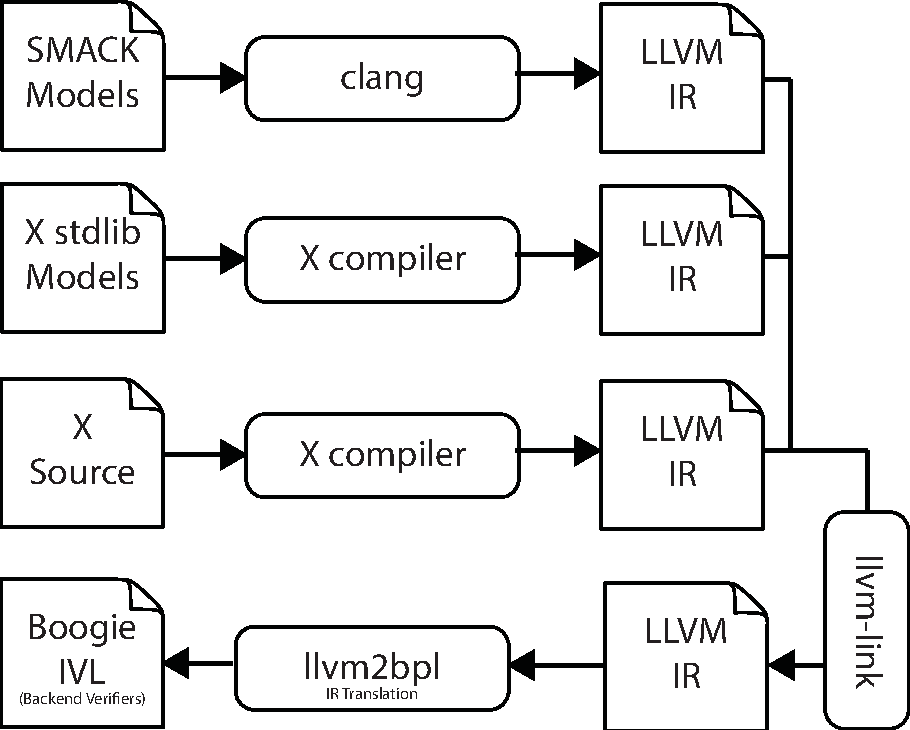
\includegraphics[width=\textwidth]{procedure}
	\caption{Toolflow for adding support for programming language X to SMACK.}
	\label{fig:vmcaixlang}
\end{figure}

%%%%%%%%%%%%%%%%%%%%%%%%%%%%%%%%%%%%%%%%%%%%%%%%%%%%%%%%%%%%%%%%%%%%%%%%%%%

\begin{figure}[H]
	\centering
	\begin{minipage}[t]{.49\textwidth}
\begin{lstlisting}[language=C,basicstyle=\ttfamily\large,commentstyle=\color{green},style=boxed]
int cap(int x) {
  int y = x;
  if (10 < x) {
    y = 10;
  }
  return y;
}

int main(void) {
  assert(cap(2)==2);
  assert(cap(15)==10);
  int x = nondet_int(); 
  assert(cap(x) <= 10);
}
\end{lstlisting}
	\end{minipage}
%
	\begin{minipage}[t]{.49\textwidth}
\begin{lstlisting}[language=swift,basicstyle=\ttfamily\large,commentstyle=\color{green},style=boxed]
func cap(_ x: Int)->Int
{
  var y = x
  if 10 < x {
    y = 10
  }
  return y
}

assert(cap(2) == 2)
assert(cap(15) == 10)
let x=Int(nondet_int())
assert(cap(x) <= 10)
\end{lstlisting}    
    \end{minipage}
	\begin{minipage}[t]{.49\textwidth}
\begin{lstlisting}[language=rust,basicstyle=\ttfamily\large,commentstyle=\color{green},style=boxed]
fn cap(x: usize)->usize
{
  let mut y = x;
  if 10 < x {
    y = 10;
  }
  return y;
}


fn main() {
  let two = cap(2);
  let ten = cap(15);
  assert!(two == 2);
  assert!(ten == 10);
  let x = nondet_int();
  assert!(x <= 10);
}
\end{lstlisting}
	\end{minipage}
%
	\begin{minipage}[t]{.49\textwidth}
\begin{lstlisting}[language=fortran,basicstyle=\ttfamily\large,commentstyle=\color{green},style=boxed]
pure function cap(x)
 integer, intent(in)::x
 integer :: cap, y
 y = x
 if (10 < y) then
   y = 10
 end if
 cap = y
end function

program main
 integer :: cap, x
 call assert(cap(2)==2)
 call assert(cap(15)==10)
 x = nondet_int()
 call assert(cap(x)<=10)
end program main
\end{lstlisting}    
    \end{minipage}
\caption{Microbenchmark with program versions in C (top left), Swift (top right), Rust (bottom left), and Fortran (bottom right).}
\label{fig:microbenchmark}
\end{figure}

%%%%%%%%%%%%%%%%%%%%%%%%%%%%%%%%%%%%%%%%%%%%%%%%%%%%%%%%%%%%%%%%%%%%%%%%%%%

\begin{figure}[H]
\begin{lstlisting}[language=fortran,basicstyle=\ttfamily\normalsize,commentstyle=\color{green},style=boxed]
program main
  use smack
  implicit none
  integer, dimension(2) :: A = (/ 2, 3 /)
  integer, dimension(2) :: B = (/ 3, 4 /)
  integer, dimension(2) :: S
  S = A + B
  call assert(S(1) == 5)
  call assert(S(2) == 7)
end program main
\end{lstlisting}
\caption{Fortran program that utilizes vectorized addition.}
\label{fig:fortran-ex}
\end{figure}

\begin{table}[H]
\caption[List of programming languages we considered and their properties]{List of programming languages we considered and their properties.
  Column \textbf{Ahead-of-Time} shows whether an Ahead-of-Time compiler
  is available for the language;
  %
  column \textbf{LLVM 3.9} indicates whether the needed LLVM version is
  supported;
  %
  column \textbf{Active} indicates whether the compiler is under active
  development, while column \textbf{Stable} indicates if there is a
  stable release;
  %
  and finally, column \textbf{Used it?} shows whether we used the language
  in our evaluation.

}
\label{tab:languages}
\centering
\setlength{\tabcolsep}{6.5pt}
\ra{2}
\vspace{1em}
\begin{tabular}{@{}lcccccc@{}}
	\toprule
	\textbf{Language} & \textbf{Compiler} & \textbf{Ahead-of-Time} & \textbf{LLVM 3.9} & \textbf{Active} & \textbf{Stable} & \textbf{Used it?} \\
	\midrule
	C & clang & \cmark & \cmark & \cmark & \cmark & \cmark \\
        \hdashline[1pt/1pt]
	C++ & clang & \cmark & \cmark & \cmark & \cmark & \cmark \\
        \hdashline[1pt/1pt]
	Fortran~\cite{flang-link} & flang & \cmark & \cmark & \cmark & \cmark & \cmark \\
        \hdashline[1pt/1pt]
	D~\cite{d-link} & ldc & \cmark & \cmark & \cmark & \cmark & \cmark \\
        \hdashline[1pt/1pt]
	Rust~\cite{rust-link} & rustc & \cmark & \cmark & \cmark & \cmark & \cmark \\
        \hdashline[1pt/1pt]
	Objective-C & clang & \cmark & \cmark & \cmark & \cmark & \cmark \\
        \hdashline[1pt/1pt]
	Swift~\cite{swift-link} & swiftc & \cmark & \cmark & \cmark & \cmark & \cmark \\
        \hdashline[1pt/1pt]
	Kotlin~\cite{kotlin-link} & kotlinc & \cmark & \cmark & \cmark & \cmark & \cmark \\
        \hdashline[1pt/1pt]
	Scala~\cite{scala-link} & scala-native & \cmark & \cmark & \cmark & \cmark & \xmark \\
        \hdashline[1pt/1pt]
	C\#~\cite{llilc} & llilc & \cmark & ? & \cmark & \cmark & \xmark \\
        \hdashline[1pt/1pt]
	Haskell~\cite{haskell-link} & ghc & \cmark & \cmark & \cmark & \cmark & \xmark \\
        \hdashline[1pt/1pt]
	Julia~\cite{julia} & julia & \xmark & \cmark & \cmark & \xmark & \xmark \\
        \hdashline[1pt/1pt]
	Go~\cite{go-link} & llgo & \cmark & \cmark & \xmark & \xmark & \xmark \\
        \hdashline[1pt/1pt]
	Python~\cite{pyston-link} & pyston & \cmark & ? & \xmark & \xmark & \xmark \\
        \hdashline[1pt/1pt]
	Ruby~\cite{ruby-link} & ruby-llvm & \cmark & \xmark & \xmark & \xmark & \xmark \\
        \hdashline[1pt/1pt]
	Java~\cite{falcon-link} & falcon (Azul) & \xmark & \xmark & \cmark & \xmark & \xmark \\
	\bottomrule
\end{tabular}
\end{table}

\begin{table}[H]
\caption[Characteristics of our microbenchmark suite]{Characteristics of our microbenchmark suite. Column \textbf{LOC} is the average
number of lines of code per benchmark across supporting languages; column \textbf{\#Lang}
is the number of languages supporting the features tested.}
\vspace{1em}
\label{tab:vmcaibenchmarks}
\centering
\setlength{\tabcolsep}{20pt}
\ra{1.75}
	\begin{tabular}{@{}lcrr@{}}
	\toprule
	\textbf{Benchmark} & \textbf{Features Tested} & \textbf{LOC} & \textbf{\#Lang} \\
	\midrule
	basic    & basic assertions & 8 & 8 \\
        \hdashline[1pt/1pt]
	compute  & integer arithmetic & 12 & 8 \\
        \hdashline[1pt/1pt]
	function & functions, if-then-else, nondet values & 19 & 8 \\
        \hdashline[1pt/1pt]
	forloop  & for loops & 14 & 8 \\
        \hdashline[1pt/1pt]
	fib      & recursion & 20 & 8 \\
        \hdashline[1pt/1pt]
	compound & objects and structures, fields & 18 & 8 \\
        \hdashline[1pt/1pt]
	array    & array creation, array access & 10 & 8 \\
        \hdashline[1pt/1pt]
	pointer  & dynamic memory allocation, references & 14 & 6 \\
        \hdashline[1pt/1pt]
	inout    & updates via side effects & 17 & 7 \\
        \hdashline[1pt/1pt]
	method   & single type dispatch & 26 & 6 \\
        \hdashline[1pt/1pt]
	dynamic  & polymorphic dispatch & 29 & 6 \\
	\bottomrule
\end{tabular}
\end{table}

\begin{table}[H]
\caption[Results of running SMACK on our microbenchmarks]{Results of running SMACK on our microbenchmarks. Symbol \cmark marks
passing, symbol \xmark failing, and \notapplic marks benchmarks that do
not have a version for the corresponding language.}
\label{tab:results}
\centering
\setlength{\tabcolsep}{9pt}
\vspace{1em}
\ra{2}
\begin{tabular}{@{}lcccccccc@{}}
\toprule
\textbf{Benchmark} & \textbf{C} & \textbf{C++} & \textbf{Objective-C} & \textbf{Rust} & \textbf{Fortran} & \textbf{D} & \textbf{Swift} & \textbf{Kotlin} \\
\midrule
basic & \cmark & \cmark & \cmark & \cmark & \cmark & \cmark & \cmark & \cmark \\
\hdashline[1pt/1pt]
compute & \cmark & \cmark & \cmark & \cmark & \cmark & \cmark & \cmark & \cmark \\
\hdashline[1pt/1pt]
function & \cmark & \cmark & \cmark & \cmark & \cmark & \cmark & \cmark & \cmark \\
\hdashline[1pt/1pt]
forloop & \cmark & \cmark & \cmark & \cmark & \cmark & \cmark & \xmark & \cmark \\
\hdashline[1pt/1pt]
fib & \cmark & \cmark & \cmark & \cmark & \cmark & \cmark & \cmark & \cmark \\
\hdashline[1pt/1pt]
compound & \cmark & \cmark & \xmark & \cmark & \cmark & \cmark & \cmark & \xmark \\
\hdashline[1pt/1pt]
array & \cmark & \cmark & \xmark & \cmark & \cmark & \cmark & \xmark & \xmark \\
\hdashline[1pt/1pt]
pointer & \cmark & \cmark & \cmark & \cmark & \cmark & \cmark & \notapplic & \notapplic \\
\hdashline[1pt/1pt]
inout & \cmark & \cmark & \cmark & \cmark & \cmark & \cmark & \cmark & \notapplic \\
\hdashline[1pt/1pt]
method & \notapplic & \cmark & \xmark & \cmark & \notapplic & \cmark & \xmark & \cmark \\
\hdashline[1pt/1pt]
dynamic & \notapplic & \xmark & \xmark & \cmark & \notapplic & \xmark & \xmark & \xmark \\
\bottomrule
\end{tabular}
\end{table}

\begin{table}[H]
\caption{Time commitment summary for adding a new language.}
\label{tab:d-exercise}
\centering
\setlength{\tabcolsep}{10pt}
\vspace{1em}
\ra{1.75}
\begin{tabular}{@{}lr@{}}
	\toprule
	\textbf{Procedure Step} & \textbf{Person-Hours} \\
	\midrule
	Write code to interoperate with SMACK models & 8 \\
	Compile and link at the LLVM IR level, test  & 3 \\
	Add and model missing functionality          & 4 \\
        \hdashline[1pt/1pt]
	\multicolumn{1}{r}{Total:}                 & 15 \\
	\bottomrule
\end{tabular}
\end{table}

\begin{table}[H]
\caption[Equivalence checking of half-precision floating-point
  implementations in C and Rust]{Equivalence checking of half-precision floating-point
  implementations in C and Rust.
  % 
%  Column \textbf{Function} shows the methods of Rust \textit{f16} type.
  %
  Column \textbf{Equal?} shows whether the two implementations
  are equivalent;
  %
  column \textbf{Time} gives the verification runtime in seconds and
  %
  column \textbf{LOC} gives the number of lines of code in the checked Rust function.
  }
  \label{tab:rust-half}
\centering
\vspace{2em}
\setlength{\tabcolsep}{8pt}
\ra{1.75}
\begin{tabular}{@{}lcrr@{}}
\toprule
\textbf{Function} & \textbf{Equal?} & \textbf{Time(s)} & \textbf{LOC} \\
\midrule
  eq        & \cmark{} & 13 & 8 \\
  lt        & \cmark{} & 22 & 13 \\
  le        & \cmark{} & 18 & 13 \\
  gt        & \cmark{} & 17 & 13 \\
  ge        & \cmark{} & 18 & 13 \\
\hdashline[1pt/1pt]
  to\_f32   & \cmark{} & 8  & 41 \\
  to\_f64   & \cmark{} & 8 & 41 \\
  from\_f32 & \xmark{} & 5 & 68 \\
  from\_f64 & \xmark{} & 4 & 70 \\
\hdashline[1pt/1pt]
  is\_nan   & \cmark{} & 4 & 3\\
\bottomrule
\end{tabular}
\end{table}


\begin{table}[H]
\caption[Sizes of models we developed for each language]{Sizes of models we developed for each language.
  Column \textbf{Model LOC} gives the size of each model
  in terms of lines of code.
}
\label{tab:model-sizes}
\vspace{1em}
\centering
\setlength{\tabcolsep}{8pt}
\ra{1.75}
\begin{tabular}{@{}lr@{}}
	\toprule
	\textbf{Language} & \textbf{Model LOC} \\
	\midrule
	C &  2566 \\
	C++ &  13 \\
	Fortran &  38 \\
	D &  0 \\
	Rust & 480 \\
	Objective-C & 0 \\
	Swift &  2 \\
	Kotlin & 17 \\
	\bottomrule
\end{tabular}
%\vspace{-3mm}
\end{table}
% \bibliographystyle{splncs04}
% \bibliography{refs}

% \end{document}

